% !TeX root = ../main.tex

\chapter{ATLAS 探测器}
ATLAS 探测器是大型强子对撞机(Large Hadron Collider,LHC)上的一个探测器,它拥有对于对撞中心接近全空间立体角的探测范围。
ATLAS 探测器是一个多用途探测器,由一个被薄超导螺线管包围的内部径迹探测器、电磁和强子量能器以及一个包含三个大型超导环形磁体的μ子谱仪组成,
其剖面图见\autoref{fig:ATLAS_Drawing_with_Labels}。
内部探测器系统处于 2 T 轴向磁场中,拥有 $\abs{\eta} < 2.5$ 范围内带电粒子径迹探测能力。
\cite{ATLAS_detector}

\begin{figure}[ht]
    \centering
    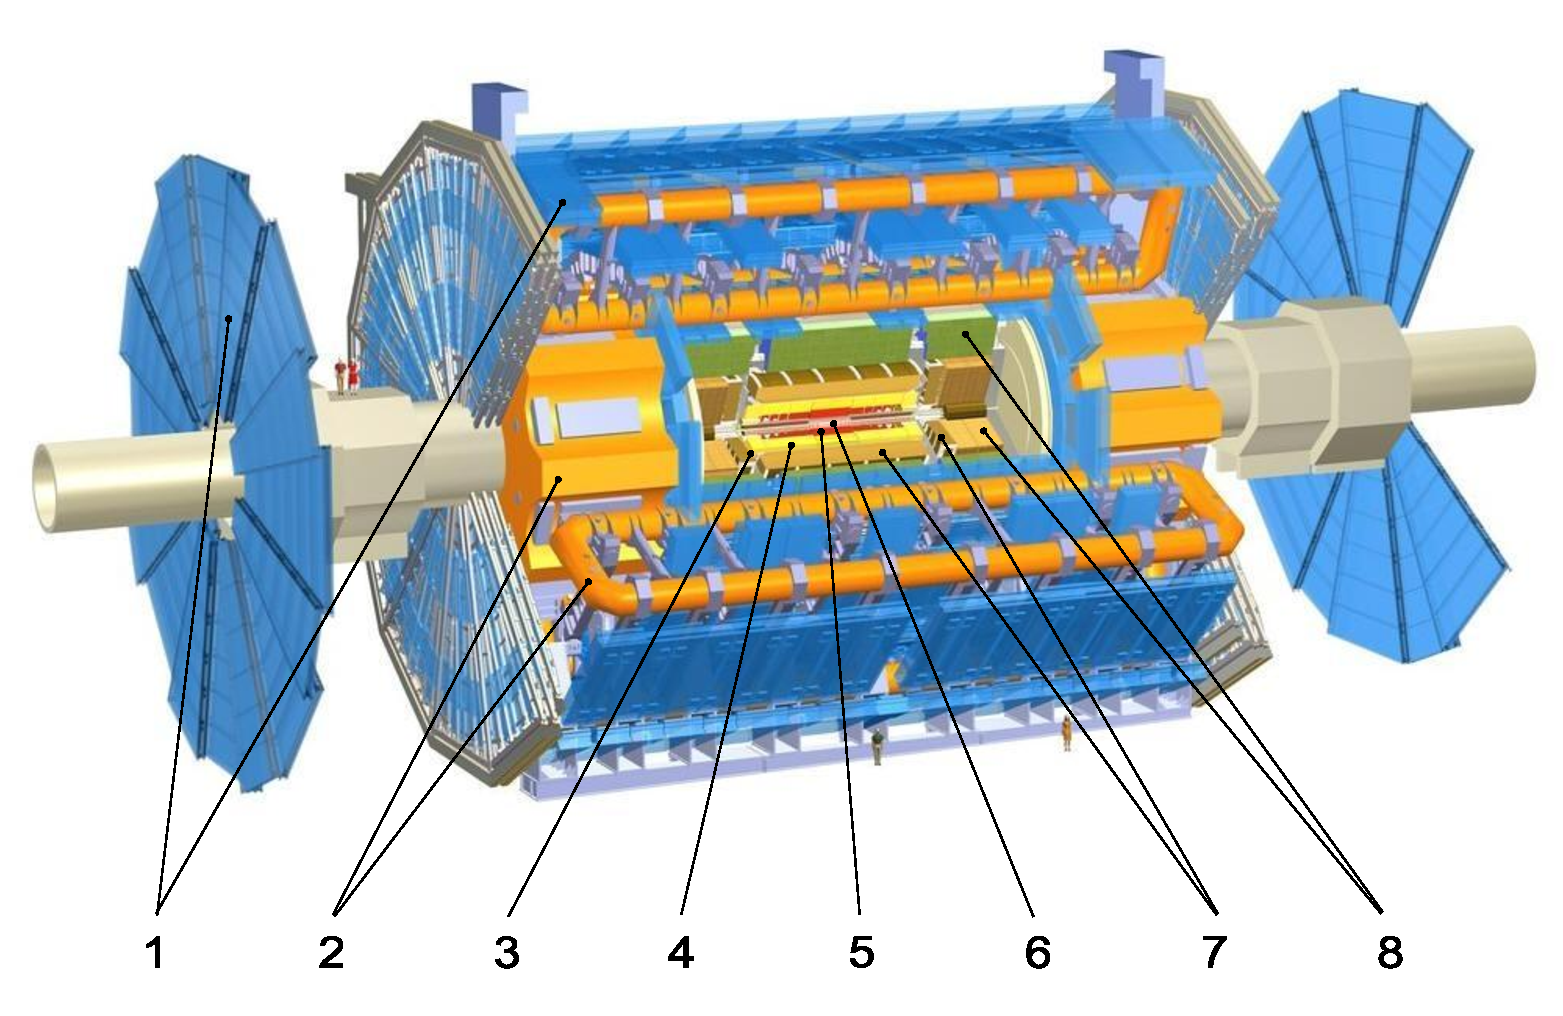
\includegraphics[width=\textwidth]{ATLAS_Drawing_with_Labels.pdf}
    \caption{ATLAS探测器剖面图}
    \label{fig:ATLAS_Drawing_with_Labels}
    \figurenote{
        μ 子谱仪:
        (1)前向区域(端盖)与桶形区域。
        磁体系统:
        (2)环形磁体,
        (3)螺线管磁体。
        内部径迹探测器:
        (4)穿越辐射探测器,
        (5)半导体探测器,
        (6)硅像素探测器。
        量能器:
        (7)液氩量能器,
        (8)瓦状量能器(tile calorimeter)。
    }
\end{figure}


\section{内部径迹探测器}
内部径迹探测器(Inner Detector)是 ATLAS 探测器最靠近束流(beam line)探测器系统,
它的主要目的是探测对撞产生的粒子在探测器中的径迹,以确定它们的位置、动量与电荷量。
内部径迹探测器的剖面图见\autoref{fig:Inner_detector},它从内到外主要分为三个部分:
硅像素探测器(Silicon Pixel Detector)、半导体探测器(Semiconductor Tracker)与穿越辐射探测器(Transition Radiation Tracker)。

\begin{figure}[ht]
    \centering
    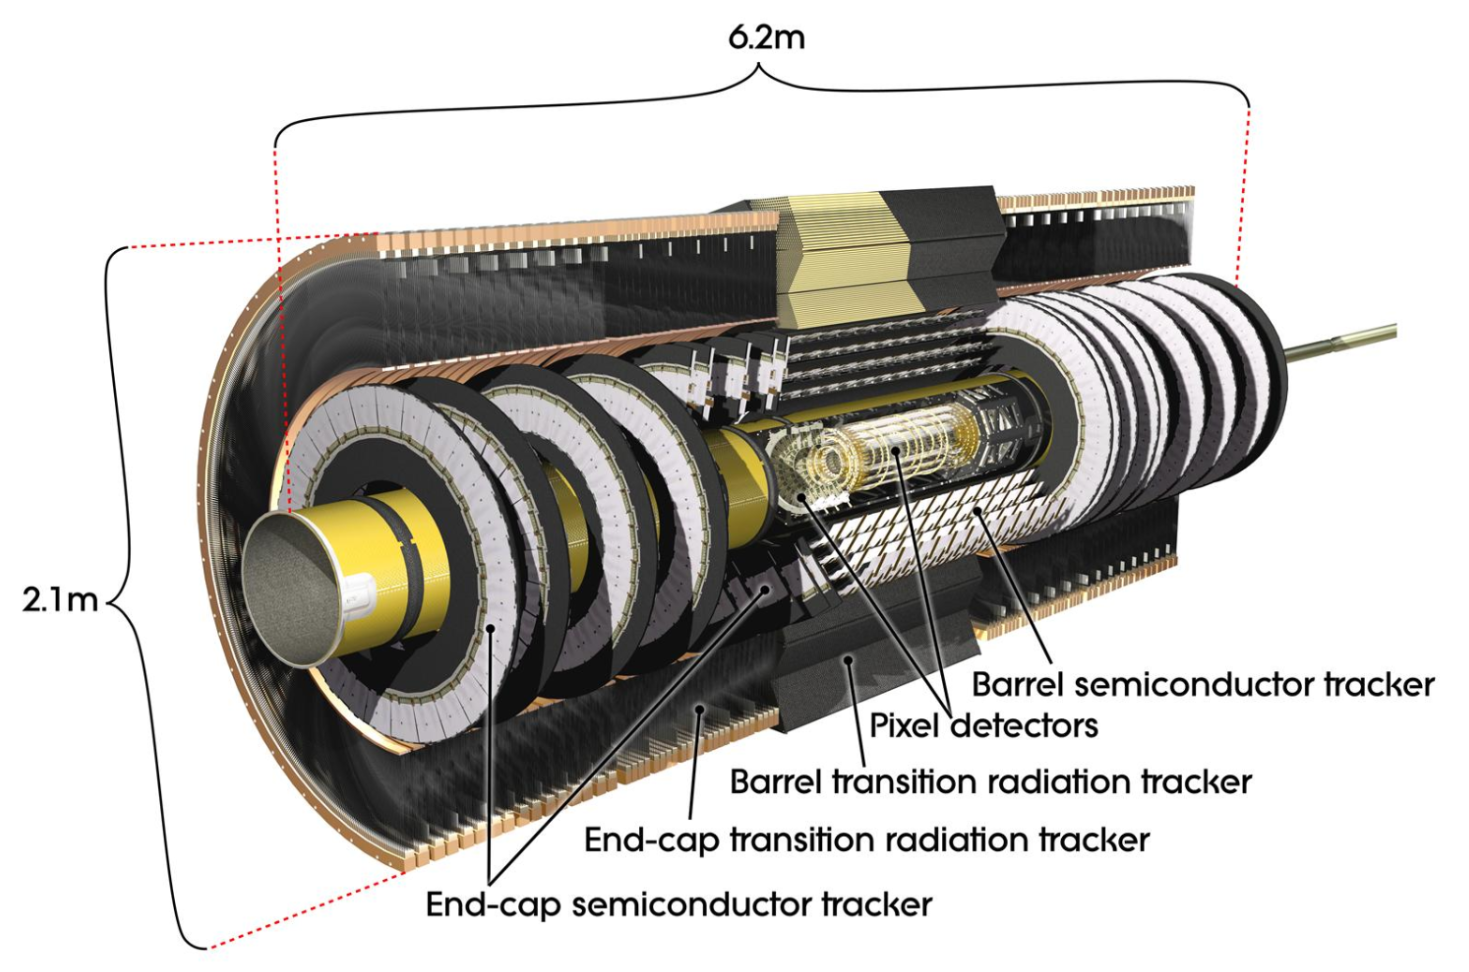
\includegraphics[width=\textwidth]{Inner_detector.png}
    \caption{内部径迹探测器剖面图}
    \label{fig:Inner_detector}
\end{figure}



\section{量能器}
由于同时存在筒部与端盖的量能器,下面两个条件之一为确定一个jet为目标CalRatio jet的必要条件:
\begin{itemize}
    \item LLP在筒部衰变:$|\eta|<1.4$且$\SI{0.5}{m}<L_{xy}<\SI{4}{m}$;
    \item LLP在端盖衰变:$|\eta|>1.4$且$\SI{2}{m}<L_{z}<\SI{6}{m}$。
\end{itemize}
其中$L_{xy}$($L_{z}$)为LLP衰变位置在$x$--$y$平面($z$轴)上与探测器中心的距离,
$\eta=-\ln \tan \frac{\theta}{2}$为喷注的赝快度。

\section{μ子探测器}
